\documentclass{beamer}
\usepackage[utf8]{inputenc}
\usepackage[T2A]{fontenc}
\usepackage[russian]{babel}
\usepackage{graphicx}

\usetheme{Madrid}
\usecolortheme{default}

\title{Модификация БД в SQL}
\author{Лазар В. И., Козлова Е. Р.}
\date{\today}

\begin{document}

% Титульный слайд
\begin{frame}
	\titlepage
\end{frame}

% Слайд: План занятия
\begin{frame}{План занятия}
	\tableofcontents
\end{frame}

% -------------------------
% Секция: Связи в БД
% -------------------------
\section{Связи в базах данных}
\begin{frame}{Зачем нужны связи?}
	\begin{itemize}
		\item \textbf{Реляционная} модель данных предполагает хранение информации в таблицах, связанных между собой.
		\item Связи (\textit{relationships}) позволяют избегать дублирования данных и повышают целостность:
		      \begin{itemize}
			      \item \textbf{One-to-One} (1:1) — например, один сотрудник --- одна личная учётная запись.
			      \item \textbf{One-to-Many} (1:N) — один отдел содержит много сотрудников.
			      \item \textbf{Many-to-Many} (M:N) — одна книга может иметь нескольких авторов и один автор — несколько книг.
		      \end{itemize}
		\item \textbf{FOREIGN KEY} — внешний ключ, указывающий на \texttt{PRIMARY KEY} другой таблицы.
		      Реализует связь и гарантирует целостность (нельзя ссылаться на несуществующую запись).
	\end{itemize}
\end{frame}

% -------------------------
% Секция: ER-модель
% -------------------------
\section{Что такое ER-модель?}
\begin{frame}{Общее представление об ER-модели}
	\begin{itemize}
		\item \textbf{ER-модель (Entity-Relationship model)} — это способ моделирования структуры базы данных
		      с помощью сущностей (Entities) и связей (Relationships).
		\item \textbf{Сущность (Entity)} — это объект реального мира, информация о котором хранится (например, «Сотрудник»).
		\item \textbf{Связь (Relationship)} — показывает, как сущности соотносятся друг с другом (1:1, 1:N, M:N).
		\item \textbf{Атрибут (Attribute)} — свойство или характеристика сущности (например, «Имя», «Зарплата»).
		\item ER-модель обычно представляют в виде диаграммы: прямоугольники — сущности,
		      ромбы (или линии с пометками) — связи, овалы — атрибуты.
		\item На основе ER-модели потом создаются таблицы и их связи (\texttt{FOREIGN KEY}) в реляционных СУБД.
	\end{itemize}
\end{frame}


\begin{frame}{Пример ER-модели}
	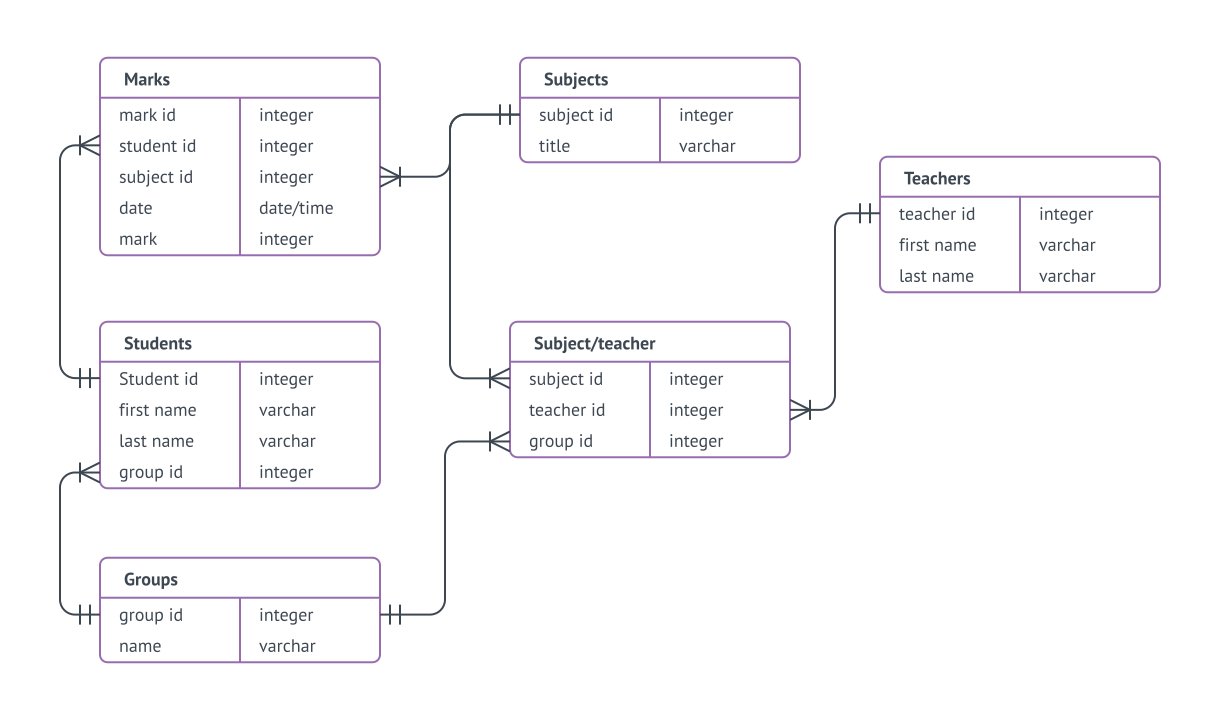
\includegraphics[scale=0.3]{er.png}
\end{frame}

% -------------------------
% Секция: CREATE, ALTER, DROP, INSERT
% -------------------------
\section{Создание, модификация и удаление таблиц}

\begin{frame}[fragile]{CREATE TABLE}
	\begin{block}{Синтаксис}
		\begin{verbatim}
CREATE TABLE table_name (
        column1 datatype [CONSTRAINT ...] [AUTOINCREMENT],
        column2 datatype [CONSTRAINT ...] [AUTOINCREMENT],
    ...
);
\end{verbatim}
	\end{block}

	\textbf{Пример}:
	\begin{verbatim}
CREATE TABLE departments (
    dept_id INTEGER PRIMARY KEY,
    dep_name VARCHAR(100) NOT NULL
);
    \end{verbatim}
\end{frame}

\begin{frame}[fragile]{FOREIGN KEY в \texttt{CREATE TABLE}}
	\textbf{Пример}:
	\begin{verbatim}
CREATE TABLE employees (
    emp_id    INTEGER PRIMARY KEY,
    emp_name  VARCHAR(50),
    position  VARCHAR(50),
    dept_id   INTEGER,
    FOREIGN KEY (dept_id)
        REFERENCES departments(dept_id)
);
    \end{verbatim}
	\textbf{Разбор}:
	\begin{itemize}
		\item Столбец \texttt{dept\_id} в \texttt{employees} ссылается на \texttt{departments.dept\_id}.
		\item При попытке вставить \texttt{dept\_id}, отсутствующий в \texttt{departments}, СУБД выдаст ошибку.
	\end{itemize}
\end{frame}

\begin{frame}[fragile]{ALTER TABLE}
	\textbf{Что можно сделать?}
	\begin{itemize}
		\item \textbf{Добавить столбец}:
		      \begin{verbatim}
ALTER TABLE table_name
ADD COLUMN new_column datatype;
\end{verbatim}

		\item \textbf{Удалить столбец}:
		      \begin{verbatim}
ALTER TABLE table_name
DROP COLUMN column_name;
\end{verbatim}

		\item \textbf{Добавить FOREIGN KEY}:
		      \begin{verbatim}
ALTER TABLE employees
ADD CONSTRAINT fk_emp_dept
FOREIGN KEY (dept_id)
REFERENCES departments(dept_id);
\end{verbatim}
	\end{itemize}
\end{frame}

\begin{frame}[fragile]{DROP TABLE}
	\begin{block}{Синтаксис}
		\begin{verbatim}
DROP TABLE table_name;
\end{verbatim}
	\end{block}

	\textbf{Особенности}:
	\begin{itemize}
		\item Удаляет таблицу целиком вместе со всеми данными.
		\item Если есть внешние ключи, может потребоваться сначала удалить связанные таблицы или отключить ограничения.
	\end{itemize}
\end{frame}

\begin{frame}[fragile]{INSERT}
	\begin{block}{Синтаксис}
		\begin{verbatim}
INSERT INTO table_name (col1, col2, ...)
VALUES (val1, val2, ...);
\end{verbatim}
	\end{block}

	\textbf{Пример}:
	\begin{verbatim}
INSERT INTO departments (dept_id, dept_name)
VALUES (1, 'Отдел продаж'),
       (2, 'Отдел разработки');
    \end{verbatim}
\end{frame}

\begin{frame}[fragile]{INSERT с учётом FOREIGN KEY}
	\begin{verbatim}
-- employees.dept_id -> departments.dept_id
INSERT INTO employees (emp_id, emp_name, position, dept_id)
VALUES
  (100, 'Иван Петров', 'Менеджер', 1),
  (101, 'Мария Сидорова', 'Разработчик', 2);

-- Если указать dept_id = 99, которого нет
-- в departments, будет ошибка
\end{verbatim}
\end{frame}

% -------------------------
% Секция: Задания
% -------------------------
\section{Задания}

\begin{frame}{Задания}
	\begin{enumerate}
		\item \textbf{Создание простой таблицы:}
		      Создайте таблицу \texttt{products} с колонками \texttt{id} (PRIMARY KEY) и \texttt{name} (VARCHAR(50), NOT NULL).

		\item \textbf{Добавление столбца:}
		      В таблицу \texttt{products} добавьте новый столбец \texttt{price} (DECIMAL(10,2)), по умолчанию равный 0.

		\item \textbf{Создание связанной таблицы:}
		      Создайте таблицу \texttt{orders} со столбцами \texttt{order\_id} (PRIMARY KEY), \texttt{product\_id} (FOREIGN KEY, ссылается на \texttt{products.id}), \texttt{quantity} (целое число).

		\item \textbf{Вставка данных:}
		      Вставьте несколько записей в таблицу \texttt{products} (например, 3-4 продукта) и в таблицу \texttt{orders} (попробуйте сослаться на существующие \texttt{product\_id}).

	\end{enumerate}
\end{frame}

\begin{frame}{Задания}
	\begin{enumerate}
		\setcounter{enumi}{4}
		\item \textbf{Проверка внешнего ключа:}
		      Убедитесь, что при попытке вставить запись в \texttt{orders} с \texttt{product\_id}, которого нет в \texttt{products}, возникает ошибка.

		\item \textbf{Изменение типа столбца:}
		      Измените тип данных \texttt{price} в \texttt{products} на \texttt{FLOAT}.


		\item \textbf{Добавление ограничения CHECK:}
		      В таблицу \texttt{products} добавьте ограничение, запрещающее ставить \texttt{price} менее 0.

		\item \textbf{Удаление столбца:}
		      Удалите столбец \texttt{quantity} из таблицы \texttt{orders}. Примечание: заранее можете подумать, не повлияет ли это на логику.
	\end{enumerate}
\end{frame}

\begin{frame}{Задания}
	\begin{enumerate}
		\setcounter{enumi}{8}
		\item \textbf{Создание таблицы со связью 1:N:}
		      Создайте таблицу \texttt{categories} (\texttt{cat\_id, cat\_name}) и добавьте в \texttt{products} столбец \texttt{cat\_id} (FOREIGN KEY), чтобы несколько продуктов могли принадлежать одной категории.

		\item \textbf{Удаление и воссоздание таблиц:}
		      Попробуйте удалить (\texttt{DROP TABLE}) таблицу \texttt{orders}, затем \texttt{products}, а затем заново воссоздать их, учитывая все необходимые FOREIGN KEY.

		\item \textbf{Использование каскадного удаления/обновления:}
		      Перед удалением таблиц измените внешние ключи \texttt{orders.product\_id} так, чтобы при удалении строки из \texttt{products} автоматически удалялись связанные строки в \texttt{orders} (\texttt{ON DELETE CASCADE}).

		\item \textbf{Добавление связанной таблицы пользователей:}
		      Создайте таблицу \texttt{users} (\texttt{user\_id}, \texttt{user\_name}, \texttt{created\_at}) и расширьте таблицу \texttt{orders}, добавив столбец \texttt{user\_id} (FOREIGN KEY). Заполните таблицу \texttt{users} несколькими записями, вставьте связанные строки в \texttt{orders}.
	\end{enumerate}
\end{frame}

\end{document}
